\section{Conceptual design options} \label{ch:options}
This chapter will discuss the five design concepts that will be considered in this report. First the selection of concepts based on the shape, mission duration and controls system design option trees is made. Finally in Section \ref{sec:conf} the five selected configurations are sketched and described. A simple load analysis is given in the form of \gls{fbd} to gain insight in the functioning of each of the concepts. The following five design are consequently used for analysis in the relevant chapters of this report.

\subsection{Concept selection}
 From the \acrfull{br} three \glspl{dot} were obtained for the design of the hypersonic decelerator. In these designs concepts; shape, mission duration and control system are considered. This yielded a set of all the individual design options. These options are shown in Fig. \ref{fig:dotshape} to \ref{fig:dotcontrol}. From these \glspl{dot} a feasible set of design options can be obtained. In Fig. \ref{fig:dotshape} six deemed feasible concept configurations can be seen. This can consequently be combined with three possible control systems from Fig. \ref{fig:dotcontrol}. The mission duration varies for all concepts and is therefore considered separately for every design concept. 

\begin{figure}[H]
%\centering
\hspace{-23mm}
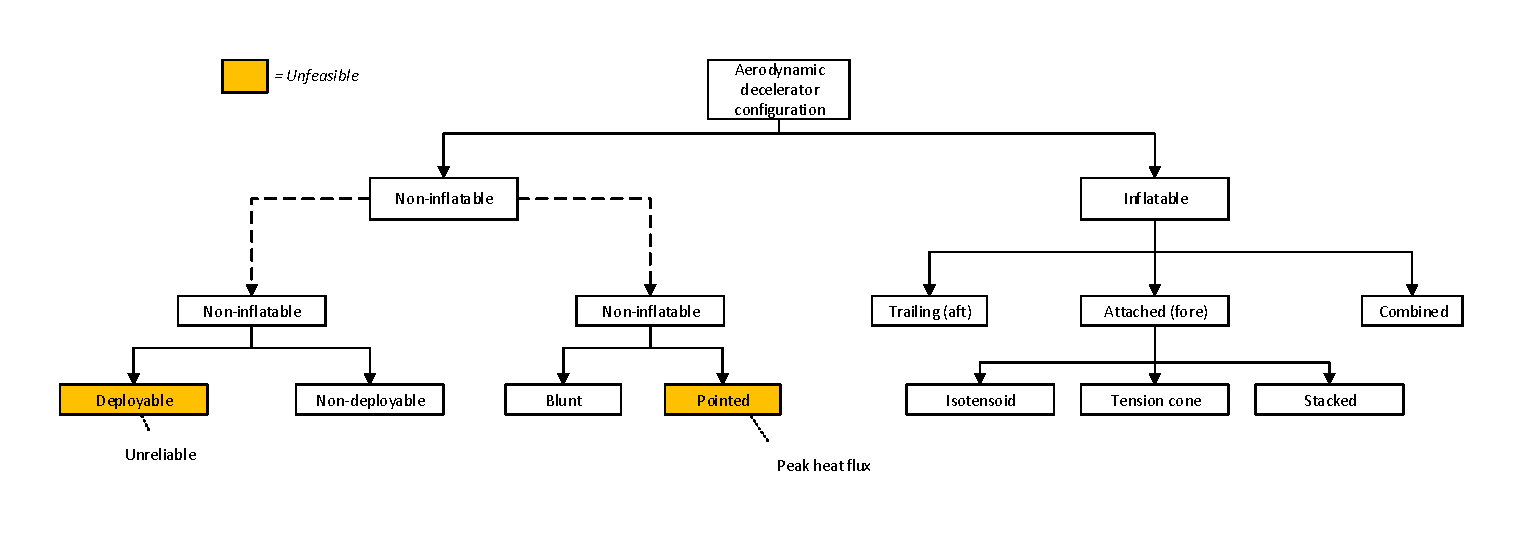
\includegraphics[width = 1.25\textwidth]{Figure/DOT_configuration.pdf}
\vspace{-5mm}
\caption{\acrlong{dot} for entry vehicle configurations}
\label{fig:dotshape}
\end{figure}

\begin{figure}[H]
\centering
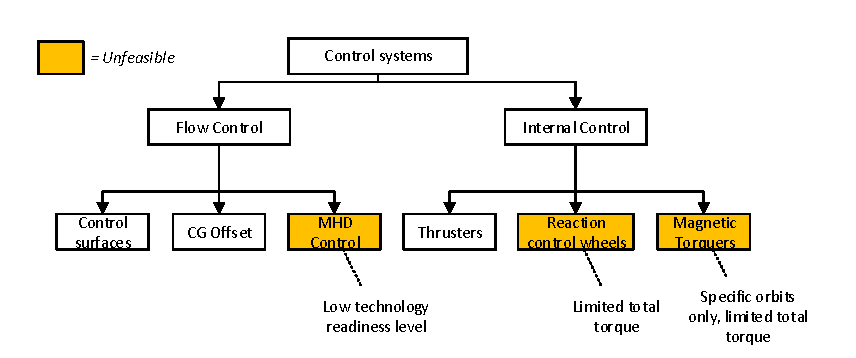
\includegraphics[width = 0.93\textwidth]{Figure/DOT_control.pdf}
\vspace{-5mm}
\caption{\acrlong{dot} for control systems}
\label{fig:dotcontrol}
\end{figure}

\begin{figure}[H]
\centering
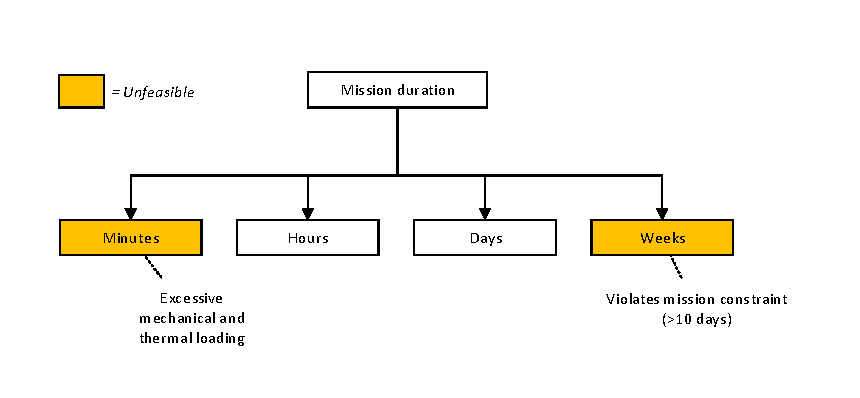
\includegraphics[width = 1.0\textwidth]{Figure/DOT_missionduration.pdf}
\vspace{-5mm}
\caption{\acrlong{dot} for mission duration}
\label{fig:dotduration}
\end{figure}

From the eighteen options yielded by combining the feasible shapes and control systems shown in Figures \ref{fig:dotshape} and \ref{fig:dotcontrol} some may be disregarded immediately since they cannot practically be combined. For obvious reasons it is crucial that each concept configuration features at least one deemed feasible control system. From this point onward the concept shape will be considered leading. 

The control systems from Fig. \ref{fig:dotcontrol} are considered separately for each of these shapes. Due to infeasibility of exotic control concepts such as the, for now, deemed infeasible \gls{mhd} the control system can be integrated with each structure as the control systems themselves do not require strict geometric properties as would be required by for example \gls{mhd} control.

Table \ref{tab:designconcepts} shows the design options that will be considered within this report. The check-marked control systems are further investigated for their feasibility and performance within Chapter \ref{ch:astrocontrol} discussing the control systems. For these control systems their performance needs to be considered separately and their feasibility must be properly supported by either references or computations. The use of a \gls{cg} offset as a control mechanism may for example be doubtful since the demonstration on its performance is only done in the \gls{irve} in which the \gls{hiad} has a relatively high mass fraction compared to the payload \cite{Dillman2012}. For this design, from the requirement CIA-Op-A02-02 (Appendix \ref{app:req}), this mass fraction is however specified to be only 10\% and effectiveness of a \gls{cg} offset as control system is therefore questionable. For other control surfaces only specific designs may be possible resulting in only the use of for example body flaps or morphing the inflatable structure as control mechanism. All these considerations are again discussed in Chapter \ref{ch:astrocontrol}. These results are finally used as one of the selection criteria in the trade off.

It must be noted that the control configurations of Table \ref{tab:designconcepts} feature the primary control mechanism. These may always be appended later on in the design process, after the trade-off, if additional control systems increase the overall systems performance. 

\begin{table}[H]
	\caption{Generation of design concepts}
	\label{tab:designconcepts}
	\centering
		\begin{tabular}{|p{0.3\textwidth}|p{0.14\textwidth}|p{0.14\textwidth}|p{0.14\textwidth}|} \hline 
			\textbf{Concept} & \textbf{Thrusters}	& \textbf{\gls{cg} offset} &  \textbf{Control surfaces} \\ \hline \hline
			Stacked toroid   & \cmark	& \cmark &  \cmark \\ \hline
			Isotensoid		 & \cmark	& \cmark &  \xmark\\ \hline
			Tension cone	 & \cmark	& \cmark &  \cmark \\ \hline
			Trailing 		 & \xmark	& \cmark &  \cmark \\ \hline
			Combined 		 & \xmark	& \cmark &  \cmark \\ \hline
			Rigid  		   	 & \cmark	& \cmark &  \cmark \\ \hline
		\end{tabular}
\end{table}

At this point it may be noted that within Table \ref{tab:designconcepts} for each shape a possible control mechanism can be considered. Rather, just three combinations are deemed infeasible. Thrusters are not considered for the trailing and combined configuration. Due to the aft elements of these designs thruster cannot be considered as the primary control mechanism. Due to the large moments of inertia (due to aft elements) and very high stability of the aft systems (e.g. compare to a parachute) thrusters cannot be considered due their inefficiency. 

For the isotensoid configuration controls surface are not deemed possible since the whole outer surface is covered by the inflatable. Controls systems such as for example body flaps can therefore not be placed. Using morphing of the structure as control surface is also considered unfeasable since again the whole outer surface is covered. 

Finally, although not deemed infeasible from Table \ref{tab:designconcepts}, the combined concept is disregarded to yield a final five concepts. It is considered to be too similar to a Trailing concept. A trailing concept will still require a heat shield in front of the payload and can therefore be considered, is some aspects, a combined configuration as well. It is therefore considered that a deployable inflatable at the front will have no additional advantage. A small deployable will have a similar performance as the trailing configuration, but features the additional complexity of the front inflation system. A large frontal inflatable will however place the aft inflatable in the wake making it effectively useless. Removing the aft declarator will however yield a "simple" stacked toroid, Isotensoid or tension cone configuration. For these reasons the trailing concept will not be considered. 


...Control department moet het hier mee eens zijn. Hier kunnen nog combinaties weg gehaald worden en naar het control chapter verplaatst worden (of andersom)... 

..Check of alle argumentatie zoals besporeken er in zit... Uiteindelijk te weing argumentatie --> Naar control chapter

\subsection{Concept configurations} \label{sec:conf}

In this section a the global configuration of each of the final five shapes is considered. They are sketched and described shortly in the sections below. Moreover a simple \gls{fbd} is provided to gain insight in, where applicable, the structural principle of each of the concepts.

\textbf{Stacked toroid}

Fig. \ref{fig:conc_stacked} and \ref{fig:fbd_stacked} show the stacked toroid concept. A stacked toroid configuration features multiple inflatables which are stacked together to form the aeroshell. These inflatables are consequently covered with a thermal protection layer. In this design the payload is placed aft of the aeroshell.\

\begin{figure}[H]
\centering
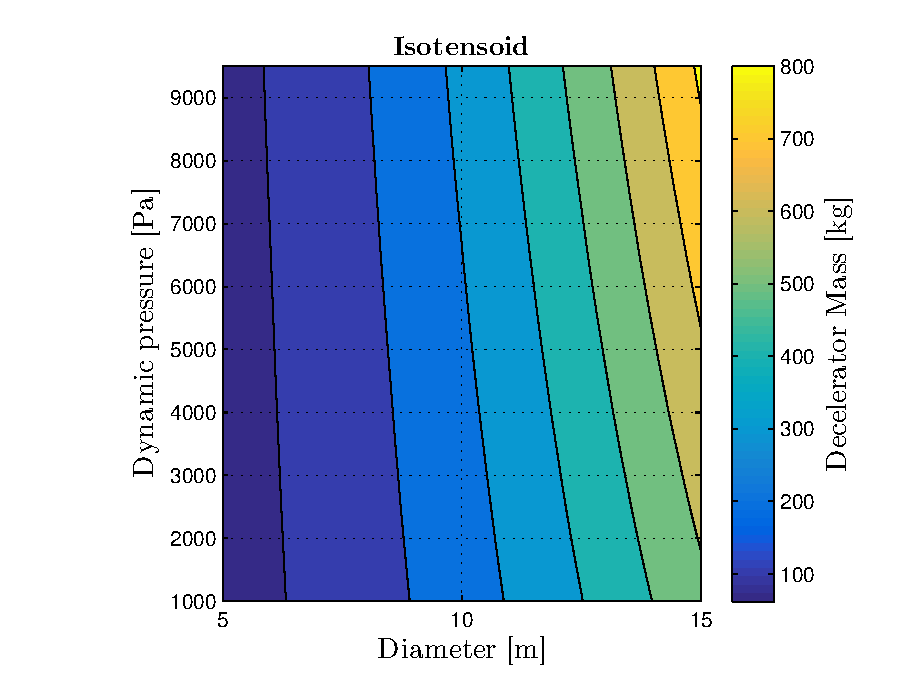
\includegraphics[width = 0.5\textwidth]{Figure/ISO_comp.eps}
\caption{A schematic view of a stacked toroid configuration}
\label{fig:conc_stacked}
\end{figure}

\begin{figure}[H]
\centering
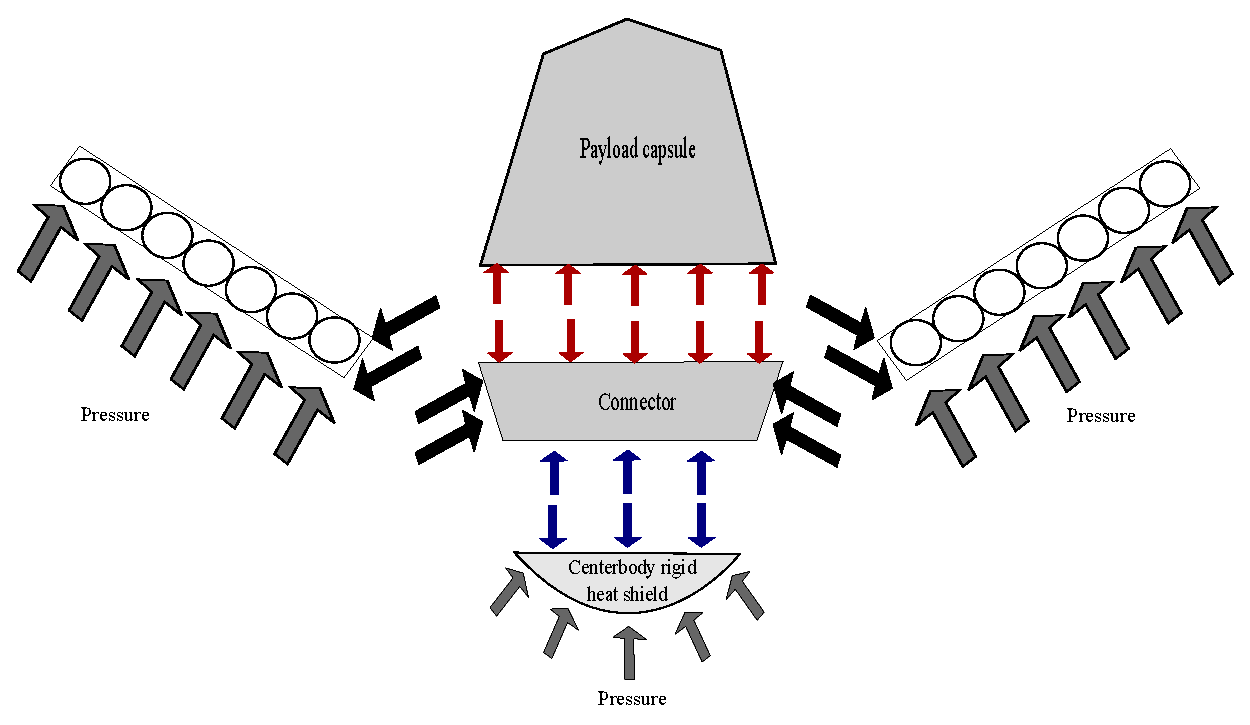
\includegraphics[width = 0.62\textwidth]{Figure/FBD_stacked.eps}
\caption{A \gls{fbd} of the stacked toroid configuration}
\label{fig:fbd_stacked}
\end{figure}


\textbf{Isotensoid}

An isotensoid configuration as displayed in Fig. \ref{fig:conc_iso} and \ref{fig:fbd_iso} features a single inflatable. This inflatable covers the whole of the payload. This inflatable is relatively large and is typically inflated using ram-air \cite{Smith2011}. 

\begin{figure}[H]
\centering
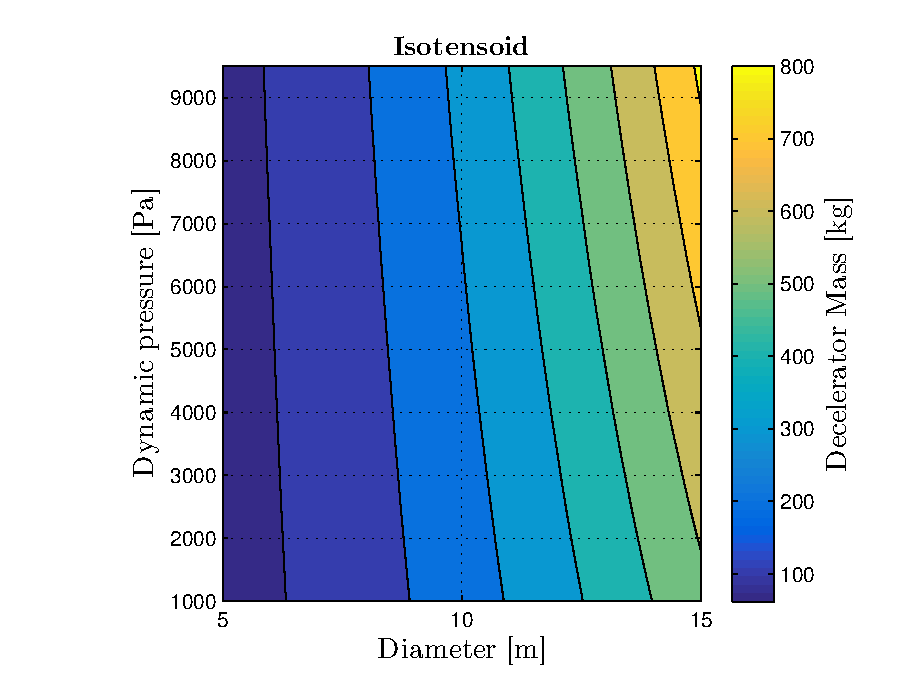
\includegraphics[width = 0.5\textwidth]{Figure/ISO_comp.eps}
\caption{A schematic view of a isotensoid configuration}
\label{fig:conc_iso}
\end{figure}

\begin{figure}[H]
\centering
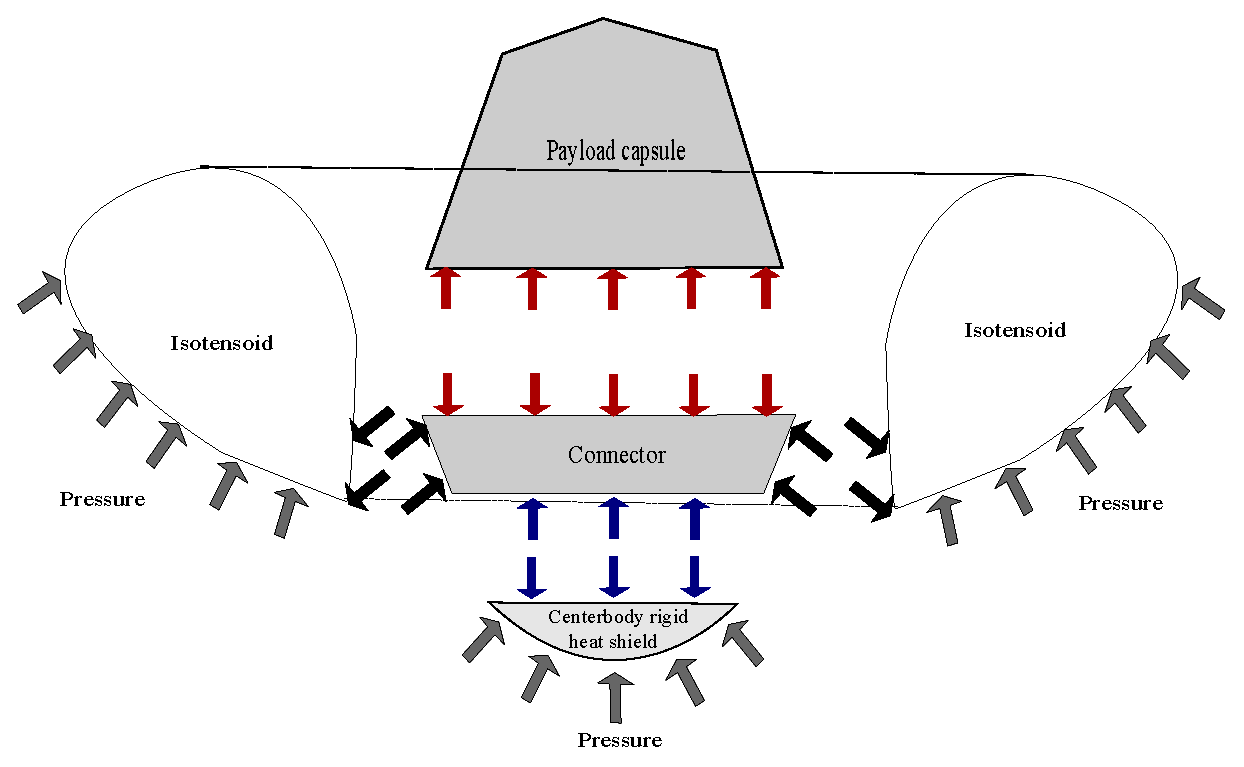
\includegraphics[width = 0.55\textwidth]{Figure/FBD_isotensoid.eps}
\caption{A \gls{fbd} of the isotensoid configuration}
\label{fig:fbd_iso}
\end{figure}

\textbf{Tension cone}

A tension cone, as shown in Fig. \ref{fig:conc_tension} and \ref{fig:fbd_tension}  again consists only of a single inflatable. In this case the inflatable is ring formed, using the ring to provide stiffness to a web spanned within. In this configuration the aeroshell is placed front of the payload, warping around it in some extend.

\begin{figure}[H]
\centering
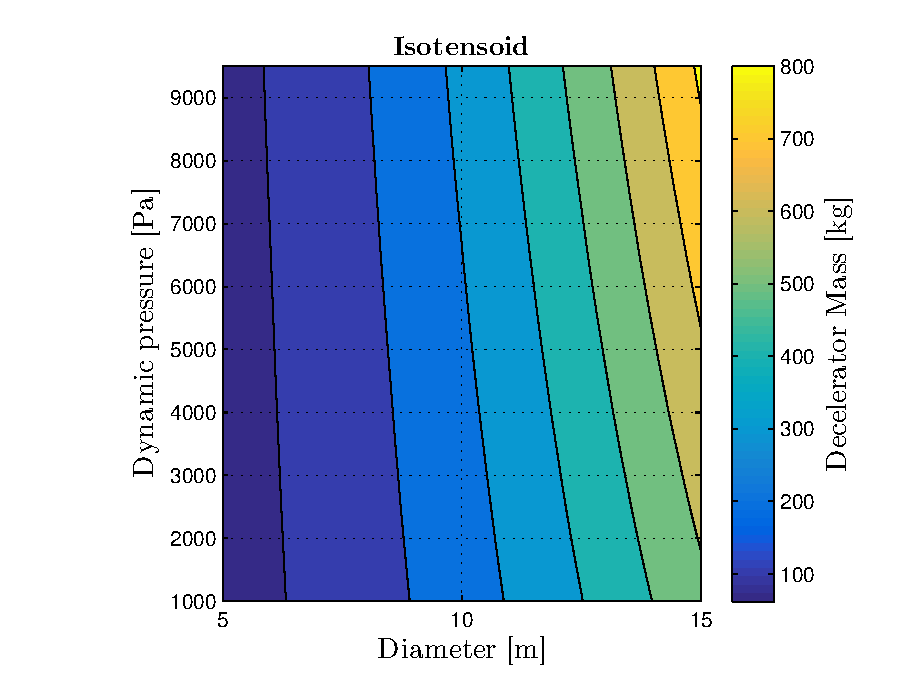
\includegraphics[width = 0.5\textwidth]{Figure/ISO_comp.eps}
\caption{A schematic view of a tension cone configuration}
\label{fig:conc_tension}
\end{figure}

\begin{figure}[H]
\centering
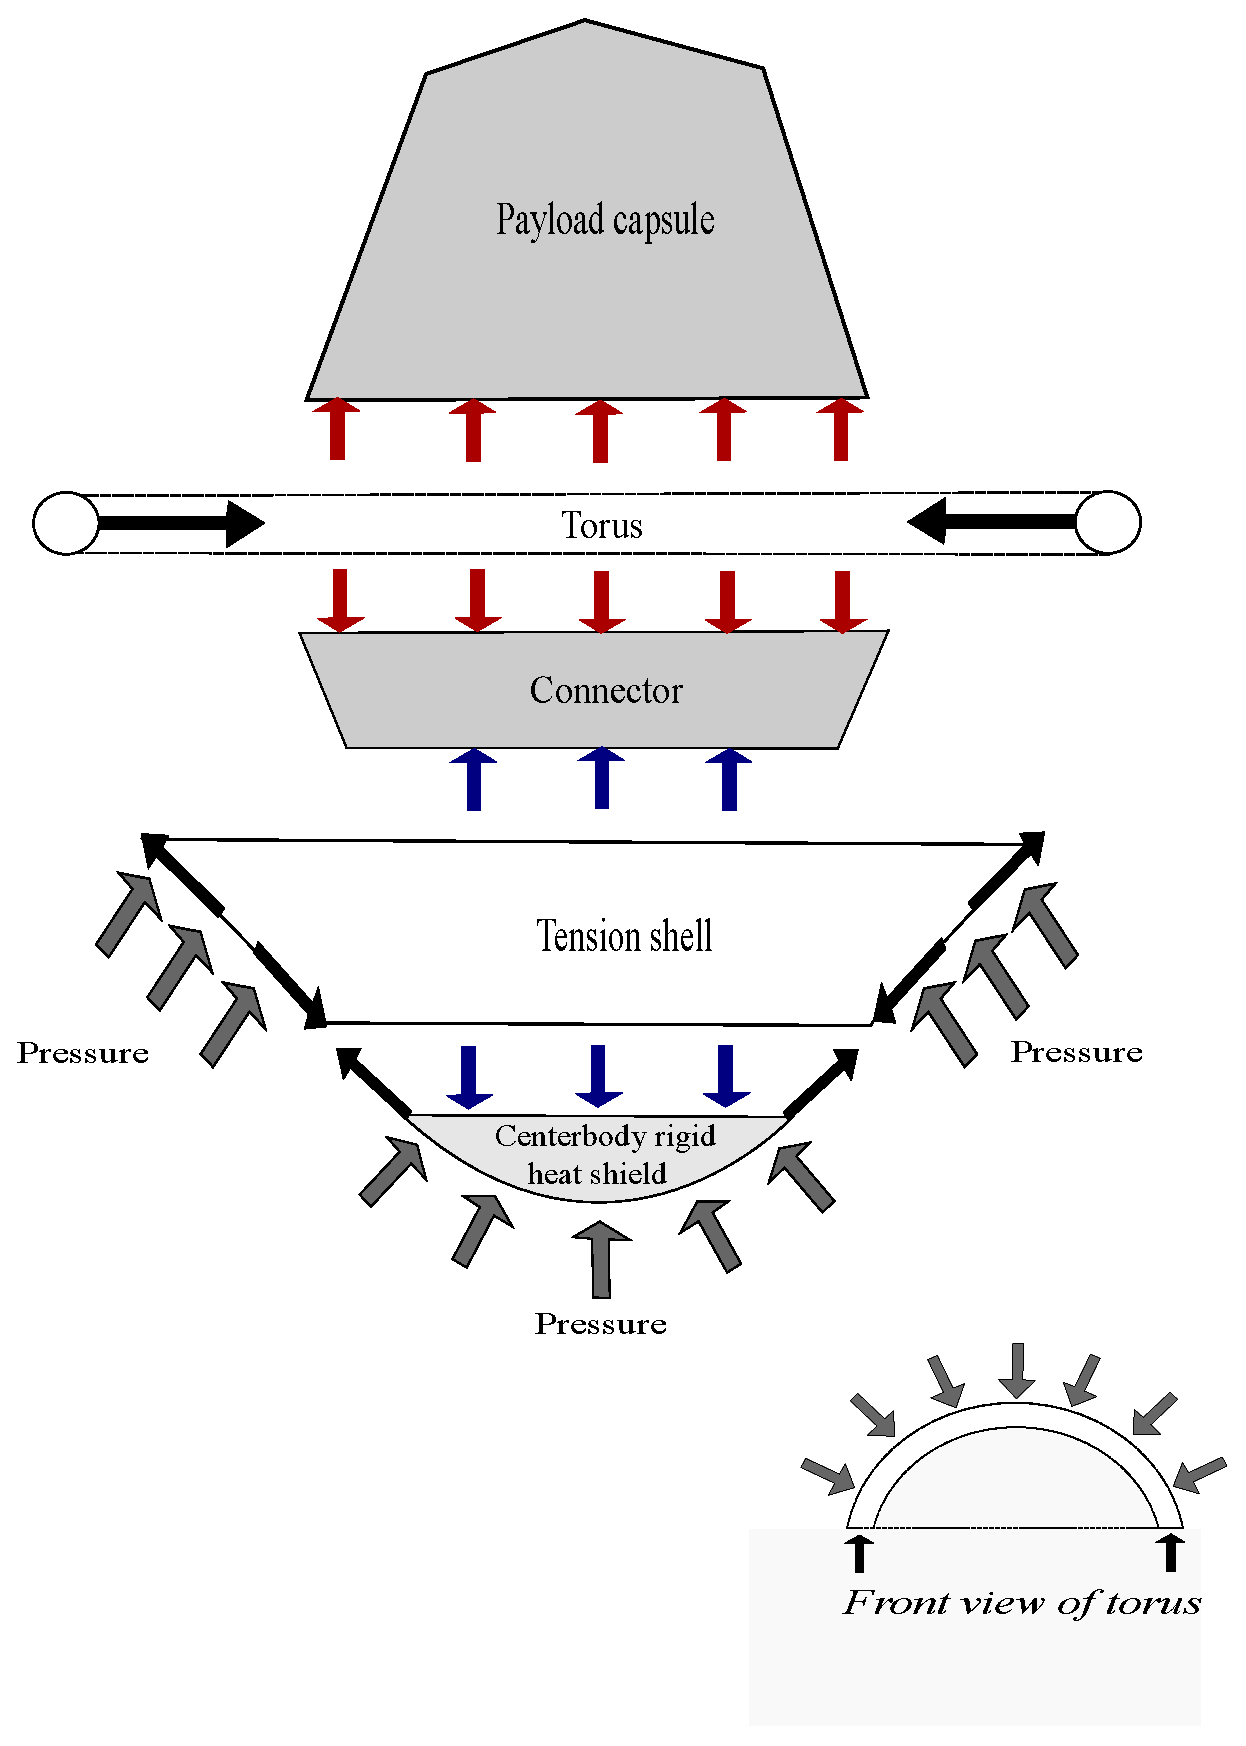
\includegraphics[width = 0.4\textwidth]{Figure/FBD_tensioncone.eps}
\caption{A \gls{fbd} of the tension cone configuration}
\label{fig:fbd_tension}
\end{figure}

\textbf{Trailing}

Fig. \ref{fig:conc_trailing} \ref{fig:fbd_trailing} show a trailing configuration. A Trailing configuration consist of two parts. A aft placed inflatable, typically referred to as the the trailing, and a front placed rigid heatshield. Since the inflatable is aft placed the payload is directly exposed to the atmosphere requiring the addition of the rigid heatshield. The shock waves induced by the front of the payload consequently create a wake aft of the payload. A typical trailing device is therefore ring formed to stay out of this wake is also displayed by Fig. \ref{fig:conc_trailing}. This is also the trailing configuration as treated within this report.

\begin{figure}[H]
\centering
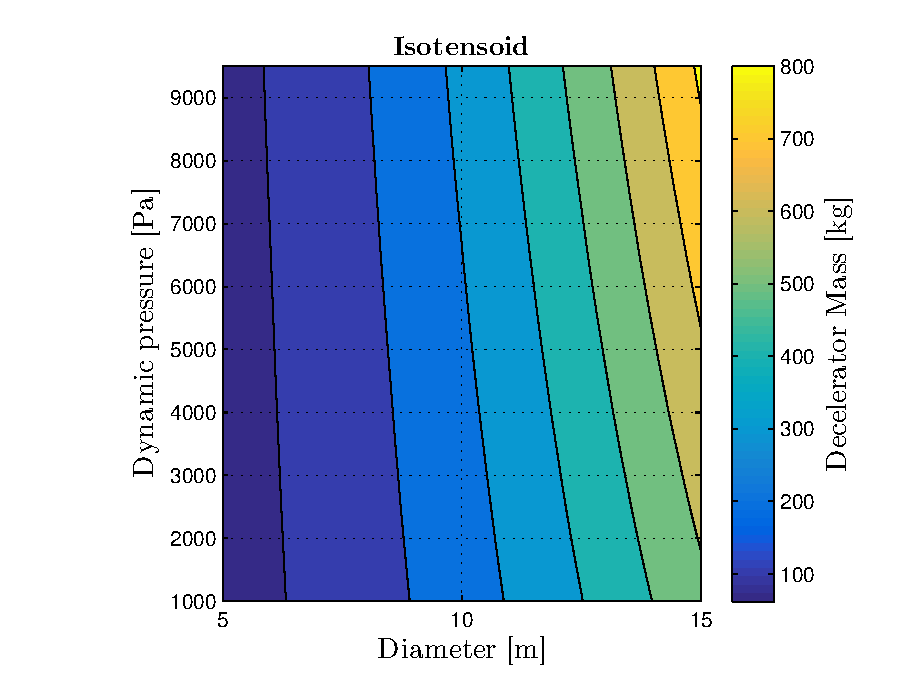
\includegraphics[width = 0.5\textwidth]{Figure/ISO_comp.eps}
\caption{A schematic view of a trailing configuration}
\label{fig:conc_trailing}
\end{figure}

\begin{figure}[H]
\centering
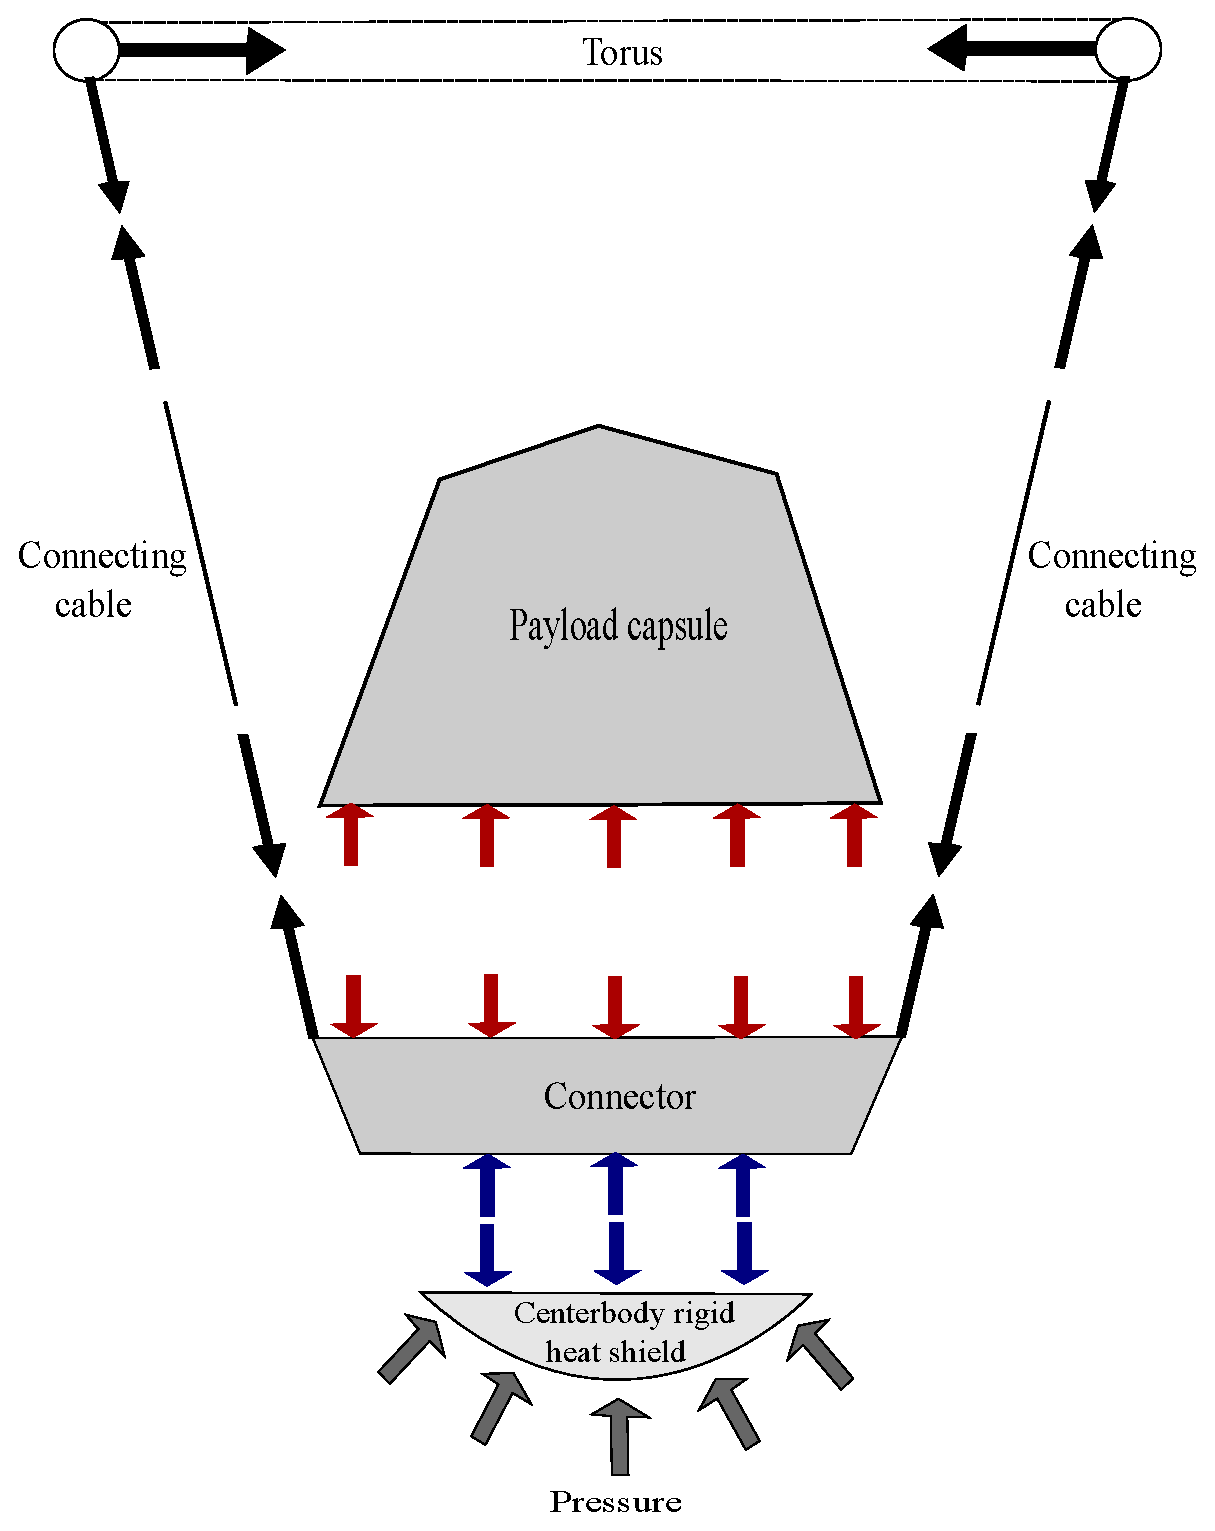
\includegraphics[width = 0.4\textwidth]{Figure/FBD_trailing.eps}
\caption{A \gls{fbd} of the trailing configuration}
\label{fig:fbd_trailing}
\end{figure}

\textbf{Rigid}

The rigid configuration is the most typical configuration and frequently used by returns to the earth atmosphere such as in the Apollo, Soyuz or planned Orion mission. Fig. \ref{fig:conc_rigid} and \ref{fig:fbd_rigid} show the Rigid configuration. This design features a rigid heatshield in front of the payload and is the only concept featuring no inflatable parts.

\begin{figure}[H]
\centering
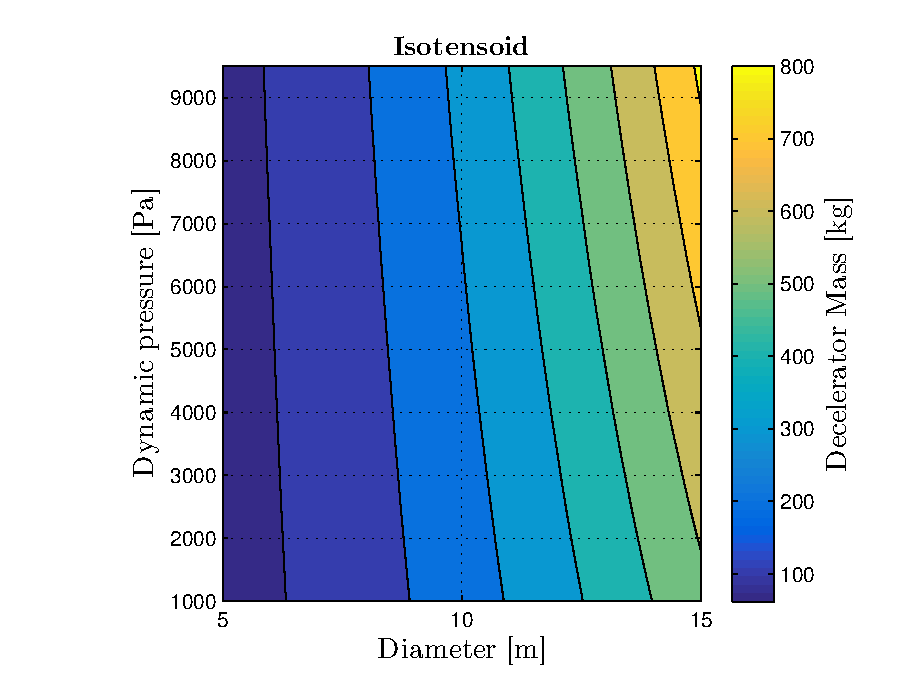
\includegraphics[width = 0.5\textwidth]{Figure/ISO_comp.eps}
\caption{A schematic view of a rigid configuration}
\label{fig:conc_rigid}
\end{figure}

\begin{figure}[H]
\centering
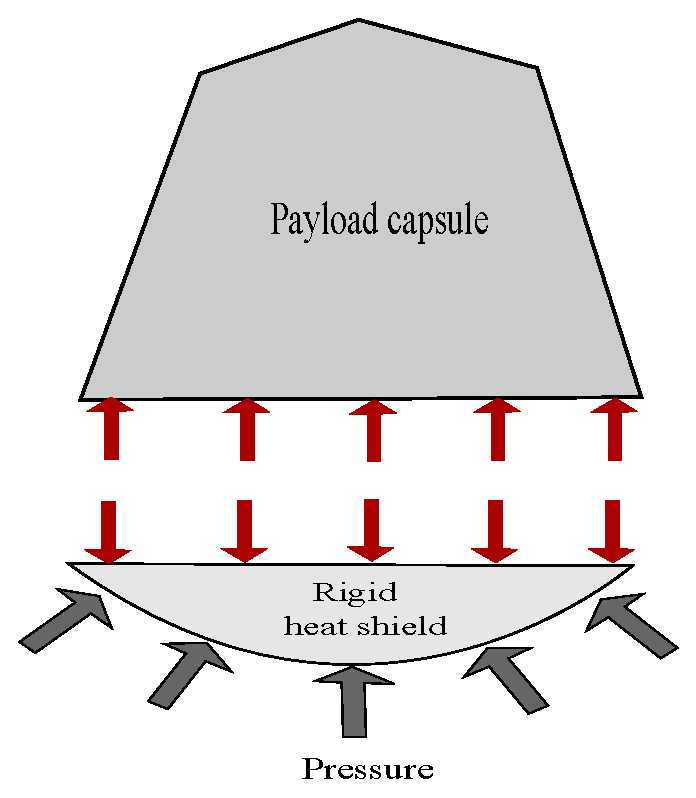
\includegraphics[width = 0.3\textwidth]{Figure/FBD_rigid.eps}
\caption{A \gls{fbd} of the rigid configuration}
\label{fig:fbd_rigid}
\end{figure}

\
